\chapter{Astrophysique}\label{ch:b3:astrophysics}

% Provenance (not for print): the astrophysics option offered across the
% surveyed third-year curricula, built here as a capstone that reuses the
% whole volume (Fermi gas -> white dwarfs, nuclear -> stellar burning,
% Planck law -> CMB, Saha -> recombination).

Chaque chapitre de ce livre répétait pour celui-ci. Les étoiles sont
des boules de gaz auto-gravitantes régies par l'hydrostatique du
volume de première année, allumées par l'effet tunnel du
\cref{ch:b3:nuclear-physics}, brillant selon la \omterm{thm:b3:photons-phonons:planck}{loi de Planck} du
\cref{ch:b3:photons-phonons}~; les étoiles mortes sont les gaz de
Fermi dégénérés du \cref{ch:b3:quantum-statistics}, à la taille de
villes~; et l'univers lui-même est un système thermique en
refroidissement dont la photographie de nourrisson --- le \omterm{def:b3:astrophysics:hubble}{fond diffus
cosmologique} --- est le corps noir le plus parfait jamais mesuré. Ce
chapitre de clôture assemble tout le volume dans le plus vaste
laboratoire possible~: comment les étoiles vivent, comment elles
meurent, ce qu'elles laissent, et comment l'univers en expansion qui
les contient a commencé, avec une physique que nous avons déjà faite.

\section{Une étoile est un équilibre}

\begin{proposition}[Équilibre hydrostatique]\label{prop:b3:astrophysics:hydrostatic}
\index{équilibre hydrostatique (stellaire)}\index{structure stellaire}
Une étoile ne s'effondre ni ne se disperse~: à chaque rayon, le
gradient de pression porte le poids du gaz au-dessus. Pour la masse
$m(r)$ contenue dans le rayon $r$,
\[
\frac{\dd P}{\dd r} = -\frac{Gm(r)\rho(r)}{r^2} .
\]
Estimé à l'échelle du Soleil entier, $P_{\text{c}} \sim GM^2/R^4 \sim
\qty{e15}{Pa}$ et, via la loi des gaz parfaits, $T_{\text{c}} \sim
10^7\,\unit{K}$ (\cref{exo:b3:astrophysics:1}) --- précisément la
température à laquelle les protons de
\cref{exo:b3:nuclear-physics:11} commencent à passer par effet
tunnel. Ce n'est pas une coïncidence mais un thermostat~: une étoile
\emph{doit} se contracter et chauffer jusqu'à ce que son cœur
s'allume, et la fusion tient alors l'équilibre pendant des millions
ou des milliards d'années. Les étoiles ont une capacité thermique
négative --- perdre de l'énergie, se contracter, devenir
\emph{plus chaude} (\cref{exo:b3:astrophysics:5}) --- et c'est
pourquoi la gravité finit toujours par gagner.
\end{proposition}

\begin{proof}
Une coquille $[r, r + \dd r]$ d'aire $A$ subit la pression $P(r)A$
par en dessous, $P(r + \dd r)A$ par au-dessus, et le poids
$g\rho A\,\dd r$ avec $g = Gm(r)/r^2$ (seule la masse intérieure
attire, par le théorème de Gauss pour la gravitation). L'équilibre
des trois donne l'équation annoncée.
\end{proof}

\begin{omfigure}
\begin{tikzpicture}[scale=1.0]
  \fill[omExo!14] (0,0) circle (2.2);
  \fill[omExo!30] (0,0) circle (1.15);
  \draw[omDef, thick] (0,0) circle (2.2);
  \draw[omDef!60] (0,0) circle (1.15);
  \node[font=\scriptsize, align=center] at (0,0)
    {cœur\\$10^7\,\unit{K}$~: fusion};
  % pressure arrows outward
  \foreach \ang in {25,115,205,295}
    \draw[->, omThm, thick] (\ang:1.25) -- (\ang:1.8);
  \node[omThm, font=\scriptsize, anchor=west] at (2.5,0.85)
    {la pression pousse dehors};
  % gravity arrows inward
  \foreach \ang in {70,160,250,340}
    \draw[->, omDef, thick] (\ang:2.75) -- (\ang:2.3);
  \node[omDef, font=\scriptsize, anchor=west] at (2.5,-0.85)
    {la gravité tire dedans};
\end{tikzpicture}

{\small Une étoile, dessinée comme son propre bilan des forces. La
fusion alimente la pression qui porte le poids propre de l'étoile~;
les deux forces négocient pendant dix milliards d'années --- et
chaque destin stellaire de ce chapitre est ce qui arrive quand l'une
d'elles est à court d'arguments.}
\end{omfigure}

\section{La vie des étoiles}

\begin{definition}[Le diagramme de Hertzsprung--Russell]\label{def:b3:astrophysics:hr}
\index{diagramme de Hertzsprung--Russell}\index{séquence principale}
Portez les étoiles selon leur température de surface (les chaudes à
\emph{gauche}, par convention) contre leur luminosité, toutes deux
issues des lois du corps noir du \cref{ch:b3:photons-phonons}, et
elles refusent de s'éparpiller~: quatre-vingt-dix pour cent se
pressent sur la \emph{séquence principale}, la bande diagonale des
brûleurs d'hydrogène, ordonnée par la seule masse --- plus lourde
signifie plus chaude \emph{et} disproportionnément plus brillante
($L \propto M^{3.5}$), donc de plus courte vie
($t \propto M/L \propto M^{-2.5}$~:
\cref{exo:b3:astrophysics:4}). Hors de la bande vivent les
exceptions et les fins du graphique~: des \emph{géantes} froides mais
énormes (en haut à droite), et des \emph{\omterm{ex:b3:quantum-statistics:dwarf}{naines blanches}} chaudes
mais minuscules (en bas à gauche) --- car à température fixée, par
$L = 4\pi R^2\sigma T^4$, la luminosité mesure la \emph{taille}. Le
diagramme HR n'est pas une carte d'espèces mais d'\emph{âges}~: le
point d'une étoile y dérive à mesure que son combustible s'épuise.
\end{definition}

\begin{omfigure}
\begin{tikzpicture}
  \begin{axis}[omaxis, axis x line=bottom, axis y line=left,
    width=9.8cm, height=6.8cm, xmin=0, xmax=10, ymin=-4.6, ymax=6.4,
    xlabel={température de surface (chaud $\to$ froid)},
    ylabel={$\log_{10}(L/L_\odot)$},
    xlabel style={at={(axis description cs:0.5,-0.08)}, anchor=north},
    xtick=\empty, ytick={-4,-2,0,2,4,6}, clip=false]
    % main sequence band
    \addplot[omDef, line width=5pt, opacity=0.28, domain=0.6:9.4]
      {5.0 - 1.05*x};
    \addplot[omDef, thick, domain=0.6:9.4] {5.0 - 1.05*x};
    % sun
    \fill[omExo] (axis cs:4.76,0) circle (2pt);
    \node[omExo, font=\scriptsize, anchor=north east] at (axis cs:4.6,-0.4)
      {Soleil};
    % giants
    \fill[omThm!25] (axis cs:8.1,3.4) ellipse (1.35 and 1.0);
    \node[omThm, font=\scriptsize] at (axis cs:8.1,3.4) {géantes};
    % white dwarfs
    \fill[gray!25] (axis cs:2.6,-3.2) ellipse (1.5 and 0.75);
    \node[font=\scriptsize] at (axis cs:2.6,-3.2) {naines blanches};
    \node[omDef, font=\scriptsize, rotate=-38, anchor=south] at
      (axis cs:2.6,2.5) {séquence principale};
  \end{axis}
\end{tikzpicture}

{\small Le \omterm{def:b3:astrophysics:hr}{diagramme de Hertzsprung--Russell}. La \omterm{def:b3:astrophysics:hr}{séquence principale}
est la bande des brûleurs d'hydrogène, une échelle de masses à lire
du haut à gauche (bleues, prodigues, mortes en quelques millions
d'années) au bas à droite (rouges, économes, survivant à l'univers
jusqu'ici). Géantes et \omterm{ex:b3:quantum-statistics:dwarf}{naines blanches} ne sont pas des bizarreries
mais des chapitres~: une même étoile visite les trois régions.}
\end{omfigure}

\begin{remark}[Comment les étoiles vieillissent, et ce qu'elles laissent]\label{rem:b3:astrophysics:evolution}
\index{géante rouge}\index{supernova}\index{nucléosynthèse (stellaire)}
Quand l'hydrogène du cœur est épuisé, la logique du thermostat
rejoue~: le cœur se contracte et chauffe, l'hélium s'allume (fusionnant
en carbone et en oxygène), l'enveloppe se gonfle d'un facteur cent ---
une \omterm{rem:b3:astrophysics:evolution}{géante rouge}. Une étoile de type solaire s'arrête là~: elle
perd son enveloppe et prend sa retraite en \omterm{ex:b3:quantum-statistics:dwarf}{naine blanche}. Une étoile
au-dessus de $\approx8M_\odot$ continue d'allumer de nouveaux
combustibles en pelures d'oignon jusqu'à ce que le cœur soit de
\emph{fer} --- le sommet de
\cref{prop:b3:nuclear-physics:binding}, d'où aucune fusion ne rend
d'énergie. Le cœur mort s'effondre en une seconde~; le rebond et le
déluge de neutrinos font voler l'étoile en éclats~: une
\emph{supernova}, qui éclipse brièvement sa galaxie, forge les
éléments au-delà du fer par capture de neutrons et diffuse le tout
dans les nuages qui bâtissent la génération suivante d'étoiles et de
planètes. Le calcium de vos os et le fer de votre sang ont suivi cette
route (\cref{pb:b3:astrophysics:1})~: la chimie est de
l'astrophysique recyclée.
\end{remark}

\section{Les cadavres~: la matière à ses limites}

\begin{proposition}[Naines blanches et étoiles à neutrons]\label{prop:b3:astrophysics:compact}
\index{naine blanche}\index{étoile à neutrons}\index{masse de Chandrasekhar}\index{trou noir}\index{rayon de Schwarzschild}
Qu'est-ce qui tient une étoile qui ne brûle plus~? La mécanique
quantique. Une \emph{\omterm{ex:b3:quantum-statistics:dwarf}{naine blanche}} est une masse solaire de carbone
et d'oxygène soutenue par sa \emph{\omterm{thm:b3:quantum-statistics:fermi}{pression de dégénérescence}
électronique} --- la pression de Fermi à $T = 0$ du
\cref{ch:b3:quantum-statistics} --- à la taille de la Terre et à une
tonne par cuillerée. Le soutien de Pauli a un plafond~: au-dessus de
la \emph{\omterm{prop:b3:astrophysics:compact}{masse de Chandrasekhar}} $M_{\text{Ch}}
\approx 1.4\,M_\odot$, les électrons deviennent relativistes et la
pression perd la course (résultat que nous énonçons sans le
démontrer). Au-delà, les électrons sont écrasés dans les protons et
une \emph{\omterm{prop:b3:astrophysics:compact}{étoile à neutrons}} se forme~: la dégénérescence des
neutrons plus la répulsion nucléaire tiennent
$\sim1.4\,M_\odot$ en une douzaine de kilomètres, à la densité
nucléaire de \cref{def:b3:nuclear-physics:nuclide} --- un noyau de la
taille d'une ville, tournant jusqu'à la milliseconde et balayant
comme un phare (un \emph{pulsar}). Et au-delà d'environ
$3\,M_\odot$, rien de connu ne résiste~: l'étoile tombe sous le rayon
où l'évasion exige la vitesse de la lumière,
\[
R_{\text{s}} = \frac{2GM}{c^2}
\qquad (\qty{3}{km}\text{ par masse solaire}) ,
\]
un \emph{\omterm{prop:b3:astrophysics:compact}{trou noir}} --- le dernier mot de la gravitation, et le pas
de porte de la relativité générale, un volume plus loin que celui-ci.
\end{proposition}
\admitted

\begin{omfigure}
\begin{tikzpicture}[scale=1.0]
  % log-scale size ladder
  \draw[omDef, fill=omExo!18, thick] (0,0) circle (1.9);
  \node[font=\scriptsize, align=center] at (0,-2.35)
    {Soleil\\$7\times10^5$ km};
  \draw[omDef, fill=omDef!15, thick] (4.4,0) circle (0.55);
  \node[font=\scriptsize, align=center] at (4.4,-2.35)
    {naine blanche\\$\sim\qty{7000}{km}$};
  \draw[omThm, fill=omThm!18, thick] (7.3,0) circle (0.16);
  \node[font=\scriptsize, align=center] at (7.3,-2.35)
    {étoile à neutrons\\$\sim\qty{12}{km}$};
  \fill (9.7,0) circle (0.06);
  \node[font=\scriptsize, align=center] at (9.7,-2.35)
    {trou noir\\$R_{\text{s}} \sim \qty{4}{km}$};
  \node[font=\scriptsize, gray, anchor=south, align=center] at (4.85,1.55)
    {masse voisine, gravité toujours plus féroce\\(tailles non à l'échelle)};
\end{tikzpicture}

{\small Une masse solaire, quatre tailles. La pression thermique
tient le Soleil~; la dégénérescence électronique la \omterm{ex:b3:quantum-statistics:dwarf}{naine blanche}~;
la dégénérescence neutronique l'\omterm{prop:b3:astrophysics:compact}{étoile à neutrons}~; rien ne tient le
\omterm{prop:b3:astrophysics:compact}{trou noir}. Chaque étape multiplie la gravité de surface par une
dizaine de milliers --- et la physique nécessaire pour s'y tenir
debout.}
\end{omfigure}

\section{L'univers en expansion}

\begin{definition}[La loi de Hubble et le commencement chaud]\label{def:b3:astrophysics:hubble}
\index{loi de Hubble}\index{fond diffus cosmologique}\index{nucléosynthèse primordiale}
Toute galaxie lointaine s'éloigne, à une vitesse proportionnelle à sa distance~:
\[
v = H_0d , \qquad H_0 \approx \qty{70}{km/s}
\text{ par mégaparsec} .
\]
Ce n'est pas une explosion \emph{dans} l'espace mais une expansion
\emph{de} l'espace --- rembobiner et tout fut jadis dense et chaud~:
il y a $1/H_0 \approx 14$ milliards d'années
(\cref{exo:b3:astrophysics:9}). L'univers primordial est ce livre
rejoué en accéléré. À une seconde, c'est une soupe de particules au
\unit{MeV} (\cref{ch:b3:particle-physics})~; dans les premières
minutes, le \cref{ch:b3:nuclear-physics} se déchaîne et fige
\emph{un quart d'hélium en masse} --- prédit par un facteur de
Boltzmann, observé partout
(\cref{exo:b3:astrophysics:11}). À 380\,000 ans et \qty{3000}{K},
l'\omterm{prop:b3:grand-canonical:saha}{équation de Saha}
(\cref{prop:b3:grand-canonical:saha}) laisse enfin les électrons se
poser sur les protons~; le brouillard se dissipe, et cette lumière
diffusée une dernière fois --- étirée d'un facteur mille par
l'expansion --- nous parvient aujourd'hui comme le \emph{fond diffus
cosmologique}~: un spectre de Planck à \qty{2.725}{K}
(\cref{ch:b3:photons-phonons}), la plus ancienne photographie qui
soit. Ce que l'image montre aussi~: les galaxies tournent et
s'agglomèrent comme si elles étaient pilotées par une \emph{\omterm{rem:b3:particle-physics:higgs}{matière
noire}} qu'aucun détecteur n'a saisie, et l'expansion \emph{accélère}
sous une \emph{énergie sombre} que personne n'a expliquée --- les
quatre-vingt-quinze pour cent du budget que ce livre ne peut encore
écrire.
\end{definition}

\begin{omfigure}
\begin{tikzpicture}
  \begin{axis}[omaxis, axis x line=bottom, axis y line=left,
    width=9.6cm, height=5.8cm, xmin=0, xmax=105, ymin=0, ymax=8.4,
    xlabel={distance (\unit{Mpc})},
    ylabel={vitesse de récession ($10^3\,\unit{km/s}$)},
    xlabel style={at={(axis description cs:0.5,-0.1)}, anchor=north},
    xtick={25,50,75,100}, ytick={2,4,6,8}, clip=true]
    \addplot[omDef, thick, domain=0:103] {0.07*x};
    \addplot[only marks, mark=*, mark size=1.4pt, omThm]
      coordinates {(9,0.75) (17,1.05) (24,1.85) (31,2.0) (39,2.9)
        (46,3.05) (54,3.95) (61,4.1) (69,5.05) (76,5.15)
        (84,6.05) (91,6.2) (98,7.0)};
    \node[omDef, font=\scriptsize, anchor=north west] at (axis cs:57,3.6)
      {pente $H_0$};
  \end{axis}
\end{tikzpicture}

{\small La \omterm{def:b3:astrophysics:hubble}{loi de Hubble}~: la vitesse de récession contre la
distance, chaque point une galaxie (vitesses issues des décalages
Doppler, \cref{ch:b3:relativistic-kinematics}~; distances issues des
chandelles standard). La pente est $H_0$~; son inverse est, en gros,
l'âge de l'univers.}
\end{omfigure}

\begin{omfigure}
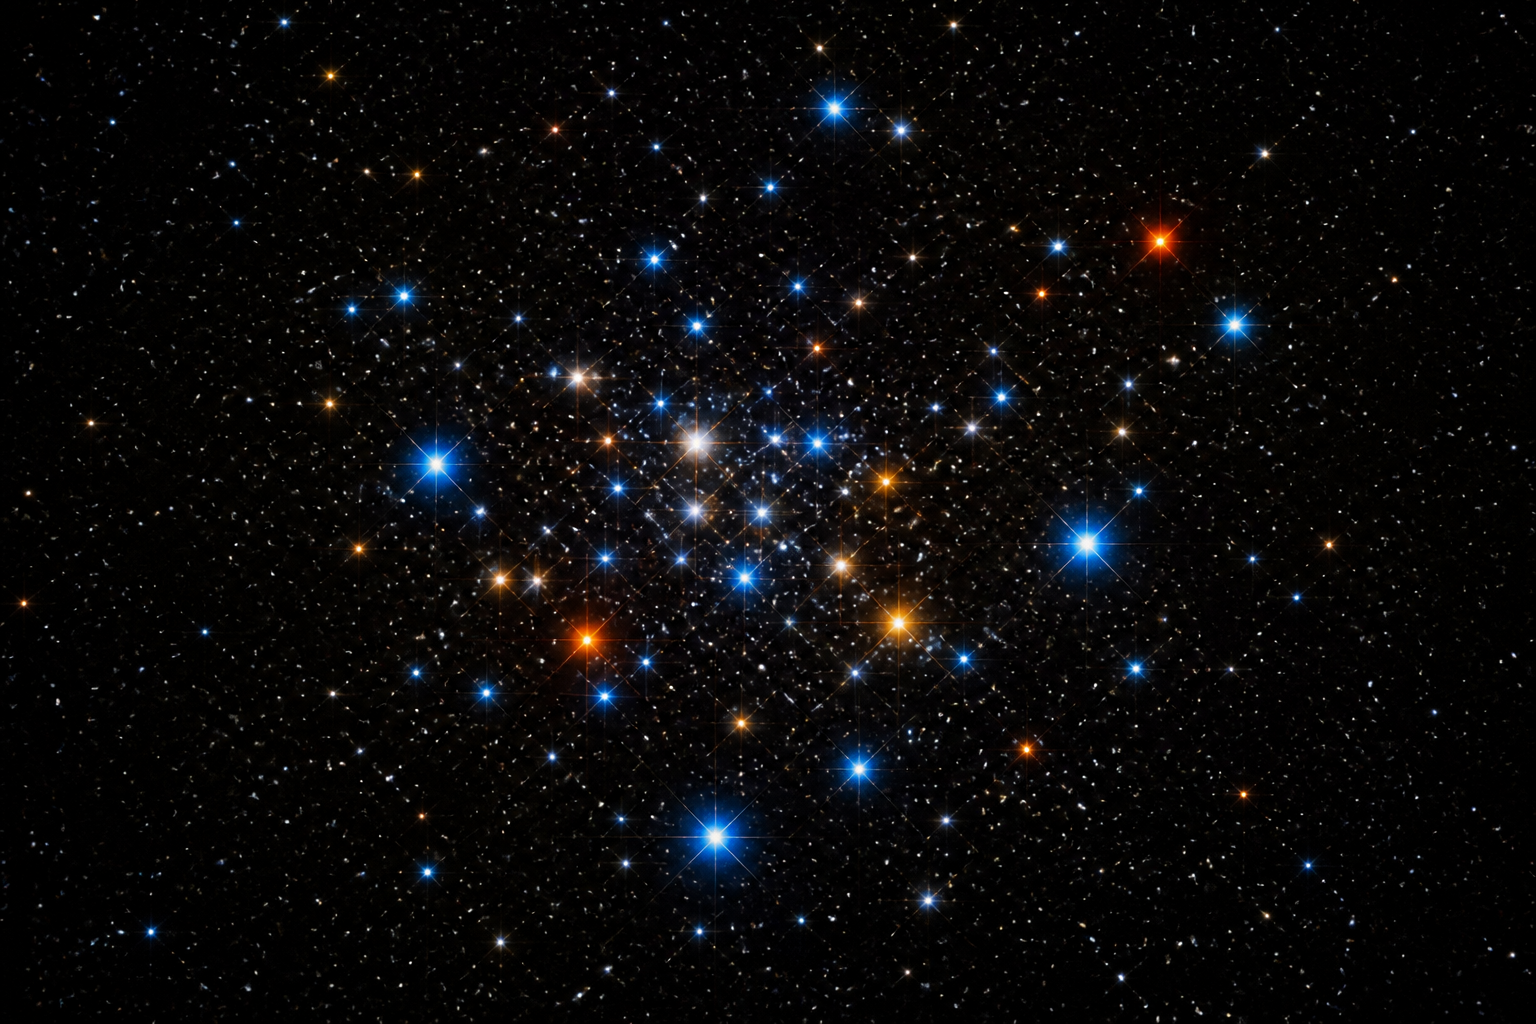
\includegraphics[width=0.58\linewidth]{images/book5/ai/b5-23-star-colors.png}

{\small Un amas ouvert~: des prodigues bleu-blanc et des naines orange économes, nées ensemble, vieillissant à des rythmes follement différents --- le \omterm{def:b3:astrophysics:hr}{diagramme de Hertzsprung--Russell}, photographié.}
\end{omfigure}

\section{Exercices}

\begin{exercise}[$\star$]\label{exo:b3:astrophysics:1}
Le Soleil, estimé. $M = \qty{2e30}{kg}$, $R = \qty{7e8}{m}$.
(a) Estimer $P_{\text{c}} \sim GM^2/R^4$. (b) Avec la masse
volumique moyenne et la loi des gaz parfaits ($P = \rho k_{\text{B}}T/
m_{\text{p}}$), estimer $T_{\text{c}}$. (c) Comparer au seuil
d'allumage $10^7\,\unit{K}$ de
\cref{exo:b3:nuclear-physics:11}. (d) Pourquoi cet accord est-il un
thermostat plutôt qu'une coïncidence~?
\end{exercise}

\begin{exercise}[$\star$]\label{exo:b3:astrophysics:2}
Peser la lumière. (a) À partir de la constante solaire
\qty{1360}{W/m^2} à $d = \qty{1.5e11}{m}$, calculer
$L_\odot$. (b) À partir de $L = 4\pi R^2\sigma T^4$, calculer la
température de surface. (c) Vérifier le maximum de Wien face au
jaune-vert visible du Soleil. (d) De quel chapitre venait la loi
employée à chaque étape~?
\end{exercise}

\begin{exercise}[$\star$]\label{exo:b3:astrophysics:3}
Lire le diagramme. Sirius B~: $T \approx \qty{25000}{K}$, $L
\approx 0.026\,L_\odot$~; Bételgeuse~: $T \approx \qty{3500}{K}$,
$L \approx 10^5\,L_\odot$. (a) Placer les deux sur le diagramme HR.
(b) À partir de $L = 4\pi R^2\sigma T^4$, calculer chaque rayon en
unités solaires. (c) Bételgeuse dans le Système solaire~: quelles
planètes sont à l'intérieur~? (d) Qu'est-ce qui doit soutenir
Sirius B~?
\end{exercise}

\begin{exercise}[$\star$]\label{exo:b3:astrophysics:4}
Vivre vite, mourir jeune. Avec $L \propto M^{3.5}$ et une durée de
vie $t \propto M/L$, et les dix milliards d'années du Soleil~: (a) la
durée de vie d'une étoile de $10\,M_\odot$~; (b) d'une naine rouge de
$0.5\,M_\odot$ --- comparer à l'âge de l'univers~; (c) pourquoi les
étoiles plus lourdes, avec \emph{plus} de combustible,
meurent-elles \emph{plus tôt}~? (d) Que la vie des astres massifs
soit brève, qu'est-ce que cela implique sur le lieu (dans une
galaxie) où surviennent les supernovae~?
\end{exercise}

\begin{exercise}[$\star\star$]\label{exo:b3:astrophysics:5}
L'étrange thermodynamique de la gravité. Pour une boule de gaz
auto-gravitante, le théorème du viriel
(\cref{ch:b3:lagrangian-mechanics}) donne une énergie totale
$E = -K$ (l'opposé de l'énergie cinétique ou thermique).
(a) En déduire~: rayonner de l'énergie rend l'étoile \emph{plus
chaude} --- une capacité thermique négative. (b) Estimer l'énergie
gravitationnelle $GM^2/R$ du Soleil. (c) Au $L_\odot$ d'aujourd'hui,
combien de temps la seule contraction aurait-elle pu l'alimenter (le
temps de Kelvin--Helmholtz)~? (d) La géologie date la Terre de
4,5 milliards d'années~: énoncer le paradoxe du dix-neuvième siècle
et sa résolution nucléaire.
\end{exercise}

\begin{exercise}[$\star\star$]\label{exo:b3:astrophysics:6}
Anatomie d'une \omterm{ex:b3:quantum-statistics:dwarf}{naine blanche}. Prendre $M = 1\,M_\odot$ à
$R = R_{\text{Terre}} = \qty{6.4e6}{m}$. (a) Calculer la masse
volumique moyenne, et la masse d'une cuillerée (\qty{5}{mL}). (b)
Calculer la gravité de surface. (c) La \omterm{thm:b3:quantum-statistics:fermi}{pression de dégénérescence} du
\cref{ch:b3:quantum-statistics} varie comme $n^{5/3}$, l'exigence de
la gravité comme $M^2/R^4 \propto n^{4/3}M^{2/3}$~: montrer que cela
implique le bizarre $R \propto M^{-1/3}$ --- les naines plus lourdes
sont \emph{plus petites}. (d) Expliquer physiquement pourquoi
entasser de la masse rétrécit l'étoile, et ce que cela annonce à la
\omterm{prop:b3:astrophysics:compact}{masse de Chandrasekhar}.
\end{exercise}

\begin{exercise}[$\star\star$]\label{exo:b3:astrophysics:7}
Anatomie d'une \omterm{prop:b3:astrophysics:compact}{étoile à neutrons}. (a) À la densité nucléaire
$\qty{2.3e17}{kg/m^3}$, calculer le rayon qui contient
$1.4\,M_\odot$. (b) Le cœur avant effondrement tournait une fois par
25 jours à $R \sim 10^5\,\unit{km}$~: utiliser la conservation du
moment cinétique pour estimer la période de rotation finale. (c)
Calculer la gravité de surface. (d) Le gel du flux amplifie le champ
magnétique comme $B \propto 1/R^2$
(\cref{ch:b3:electromagnetism-in-matter})~: à partir d'un
\qty{e-2}{T} stellaire, quel champ de surface en résulte, et pourquoi
les pulsars balaient-ils un faisceau~?
\end{exercise}

\begin{exercise}[$\star\star$]\label{exo:b3:astrophysics:8}
Le point de non-retour. (a) Obtenir $R_{\text{s}} = 2GM/c^2$ de la
condition newtonienne de vitesse de libération
$v_{\text{esc}} = c$ (la dérivation honnête exige la relativité
générale~; la réponse, fameusement, coïncide). (b) Évaluer pour le
Soleil et pour la Terre. (c) Le \omterm{prop:b3:astrophysics:compact}{trou noir} central de la Galaxie~:
$M = 4\times10^6\,M_\odot$ --- calculer $R_{\text{s}}$ et comparer à
la distance Soleil--Mercure ($\qty{5.8e10}{m}$). (d) Montrer que la
masse volumique moyenne à l'intérieur de $R_{\text{s}}$ décroît comme
$1/M^2$ --- un \omterm{prop:b3:astrophysics:compact}{trou noir} assez grand est moins dense que l'eau~: que
dit cela des intuitions d'«~écrasement~»~?
\end{exercise}

\begin{exercise}[$\star\star\star$]\label{exo:b3:astrophysics:9}
Arithmétique de Hubble. $H_0 = \qty{70}{km/s}$ par Mpc~; $1\,
\text{Mpc} = \qty{3.09e22}{m}$. (a) Convertir $H_0$ en SI. (b)
Calculer $1/H_0$ en années. (c) Une galaxie à \qty{200}{Mpc}~: sa
vitesse de récession, et le facteur d'étirement de la longueur d'onde
de sa lumière (Doppler aux petits $z$,
\cref{ch:b3:relativistic-kinematics}). (d) Pourquoi $1/H_0$ n'est-il
qu'approximativement l'âge de l'univers --- qu'a fait le taux
d'expansion entretemps~?
\end{exercise}

\begin{exercise}[$\star\star\star$]\label{exo:b3:astrophysics:10}
La plus ancienne lumière. Le fond diffus est un corps noir à
\qty{2.725}{K}. (a) Calculer sa longueur d'onde de maximum
(\cref{ch:b3:photons-phonons}) et justifier le mot
«~micro-onde~». (b) Il a été émis comme une lumière à \qty{3000}{K}~:
quel facteur d'expansion l'a étirée, et pourquoi \qty{3000}{K}
(rappeler Saha, \cref{prop:b3:grand-canonical:saha})~? (c) Sa densité
de photons vaut $\sim\qty{4e8}{m^{-3}}$~: comparer à la densité de
\omterm{def:b3:particle-physics:zoo}{baryons}, $\sim\qty{0.25}{m^{-3}}$, et donner le rapport photons sur
\omterm{def:b3:particle-physics:zoo}{baryons}. (d) Une vérification de table classique~: quelques pour cent
de la neige d'un téléviseur analogique non réglé étaient le fond
diffus --- pourquoi une antenne, pointée n'importe où, le
reçoit-elle~?
\end{exercise}

\begin{exercise}[$\star\star\star$]\label{exo:b3:astrophysics:11}
Un quart d'hélium, à partir d'un facteur de Boltzmann. Vers $t \sim
\qty{1}{s}$, $T \sim \qty{e10}{K}$ ($k_{\text{B}}T \approx
\qty{0.8}{MeV}$), le gel des réactions faibles a laissé le rapport
neutrons sur protons à sa valeur de Boltzmann
(\cref{ch:b3:canonical-ensemble}). (a) Avec $\Delta mc^2 =
\qty{1.29}{MeV}$, calculer $n/p$ au gel. (b) La désintégration des
neutrons pendant les premières minutes l'a rogné à $\approx1/7$~:
montrer que lier chaque survivant dans de l'$^4$He donne une fraction
\emph{massique} d'hélium $2(n/p)/(1 + n/p) = 25\,\%$. (c) Dites
pourquoi ce nombre, mesuré dans les étoiles partout, est une preuve
puissante du commencement chaud. (d) Pourquoi la cuisine primordiale
s'est-elle arrêtée à l'hélium (avec des traces de lithium), laissant
le carbone et tout le reste à \cref{rem:b3:astrophysics:evolution}~?
\end{exercise}

\begin{exercise}[$\star\star\star$]\label{exo:b3:astrophysics:12}
La matière manquante. La vitesse de rotation d'une galaxie spirale
reste plate à $v = \qty{220}{km/s}$ jusqu'à $r = \qty{50}{kpc}$
($\qty{1.5e21}{m}$), bien au-delà de son bord visible. (a) Pour une
orbite circulaire, montrer que $M(r) = v^2r/G$. (b) Évaluer à
\qty{50}{kpc}, en masses solaires. (c) Les étoiles et le gaz visibles
totalisent $\sim5\times10^{10}\,M_\odot$~: quelle fraction cela
explique-t-il~? (d) L'attente képlérienne au-delà du bord visible est
$v \propto r^{-1/2}$ (le schéma du Système solaire)~: qu'implique la
platitude sur la répartition de la masse invisible~?
\end{exercise}

\begin{omfigure}
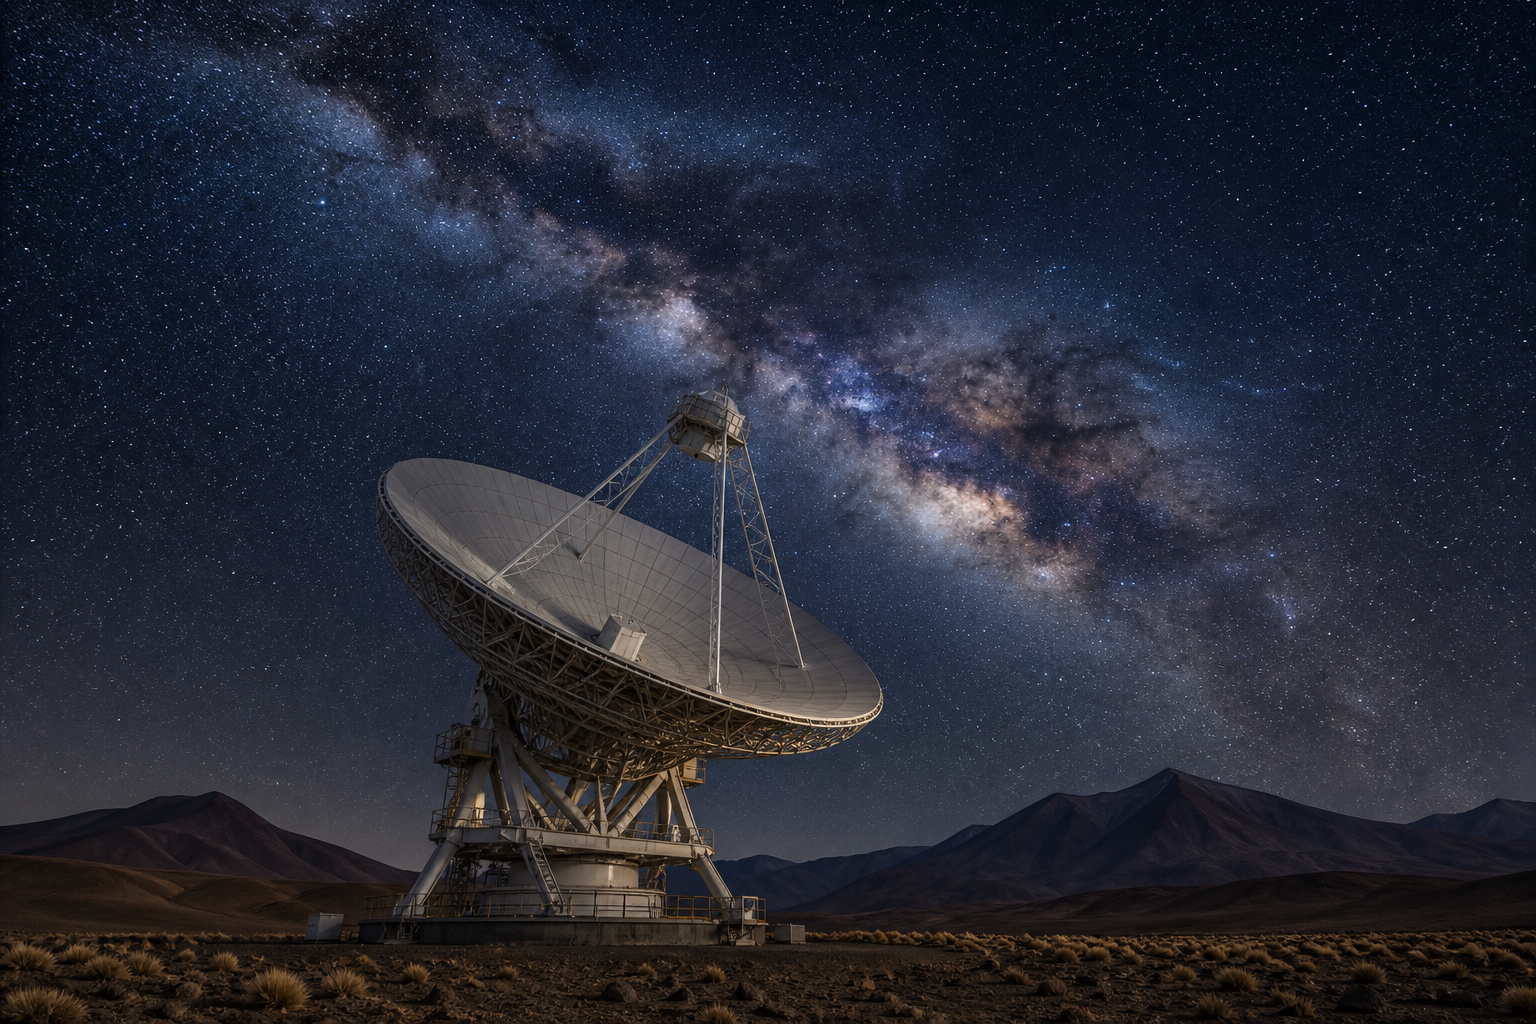
\includegraphics[width=0.58\linewidth]{images/book5/ai/b5-10-radio-dish.png}

{\small Une antenne millimétrique sous la Voie lactée~: la galaxie qu'elle écoute, suspendue au-dessus d'elle. La radioastronomie a trouvé le \omterm{def:b3:astrophysics:hubble}{fond diffus cosmologique} --- le souffle à \qty{2.7}{K} qui s'est avéré être le commencement.}
\end{omfigure}

\begin{omfigure}
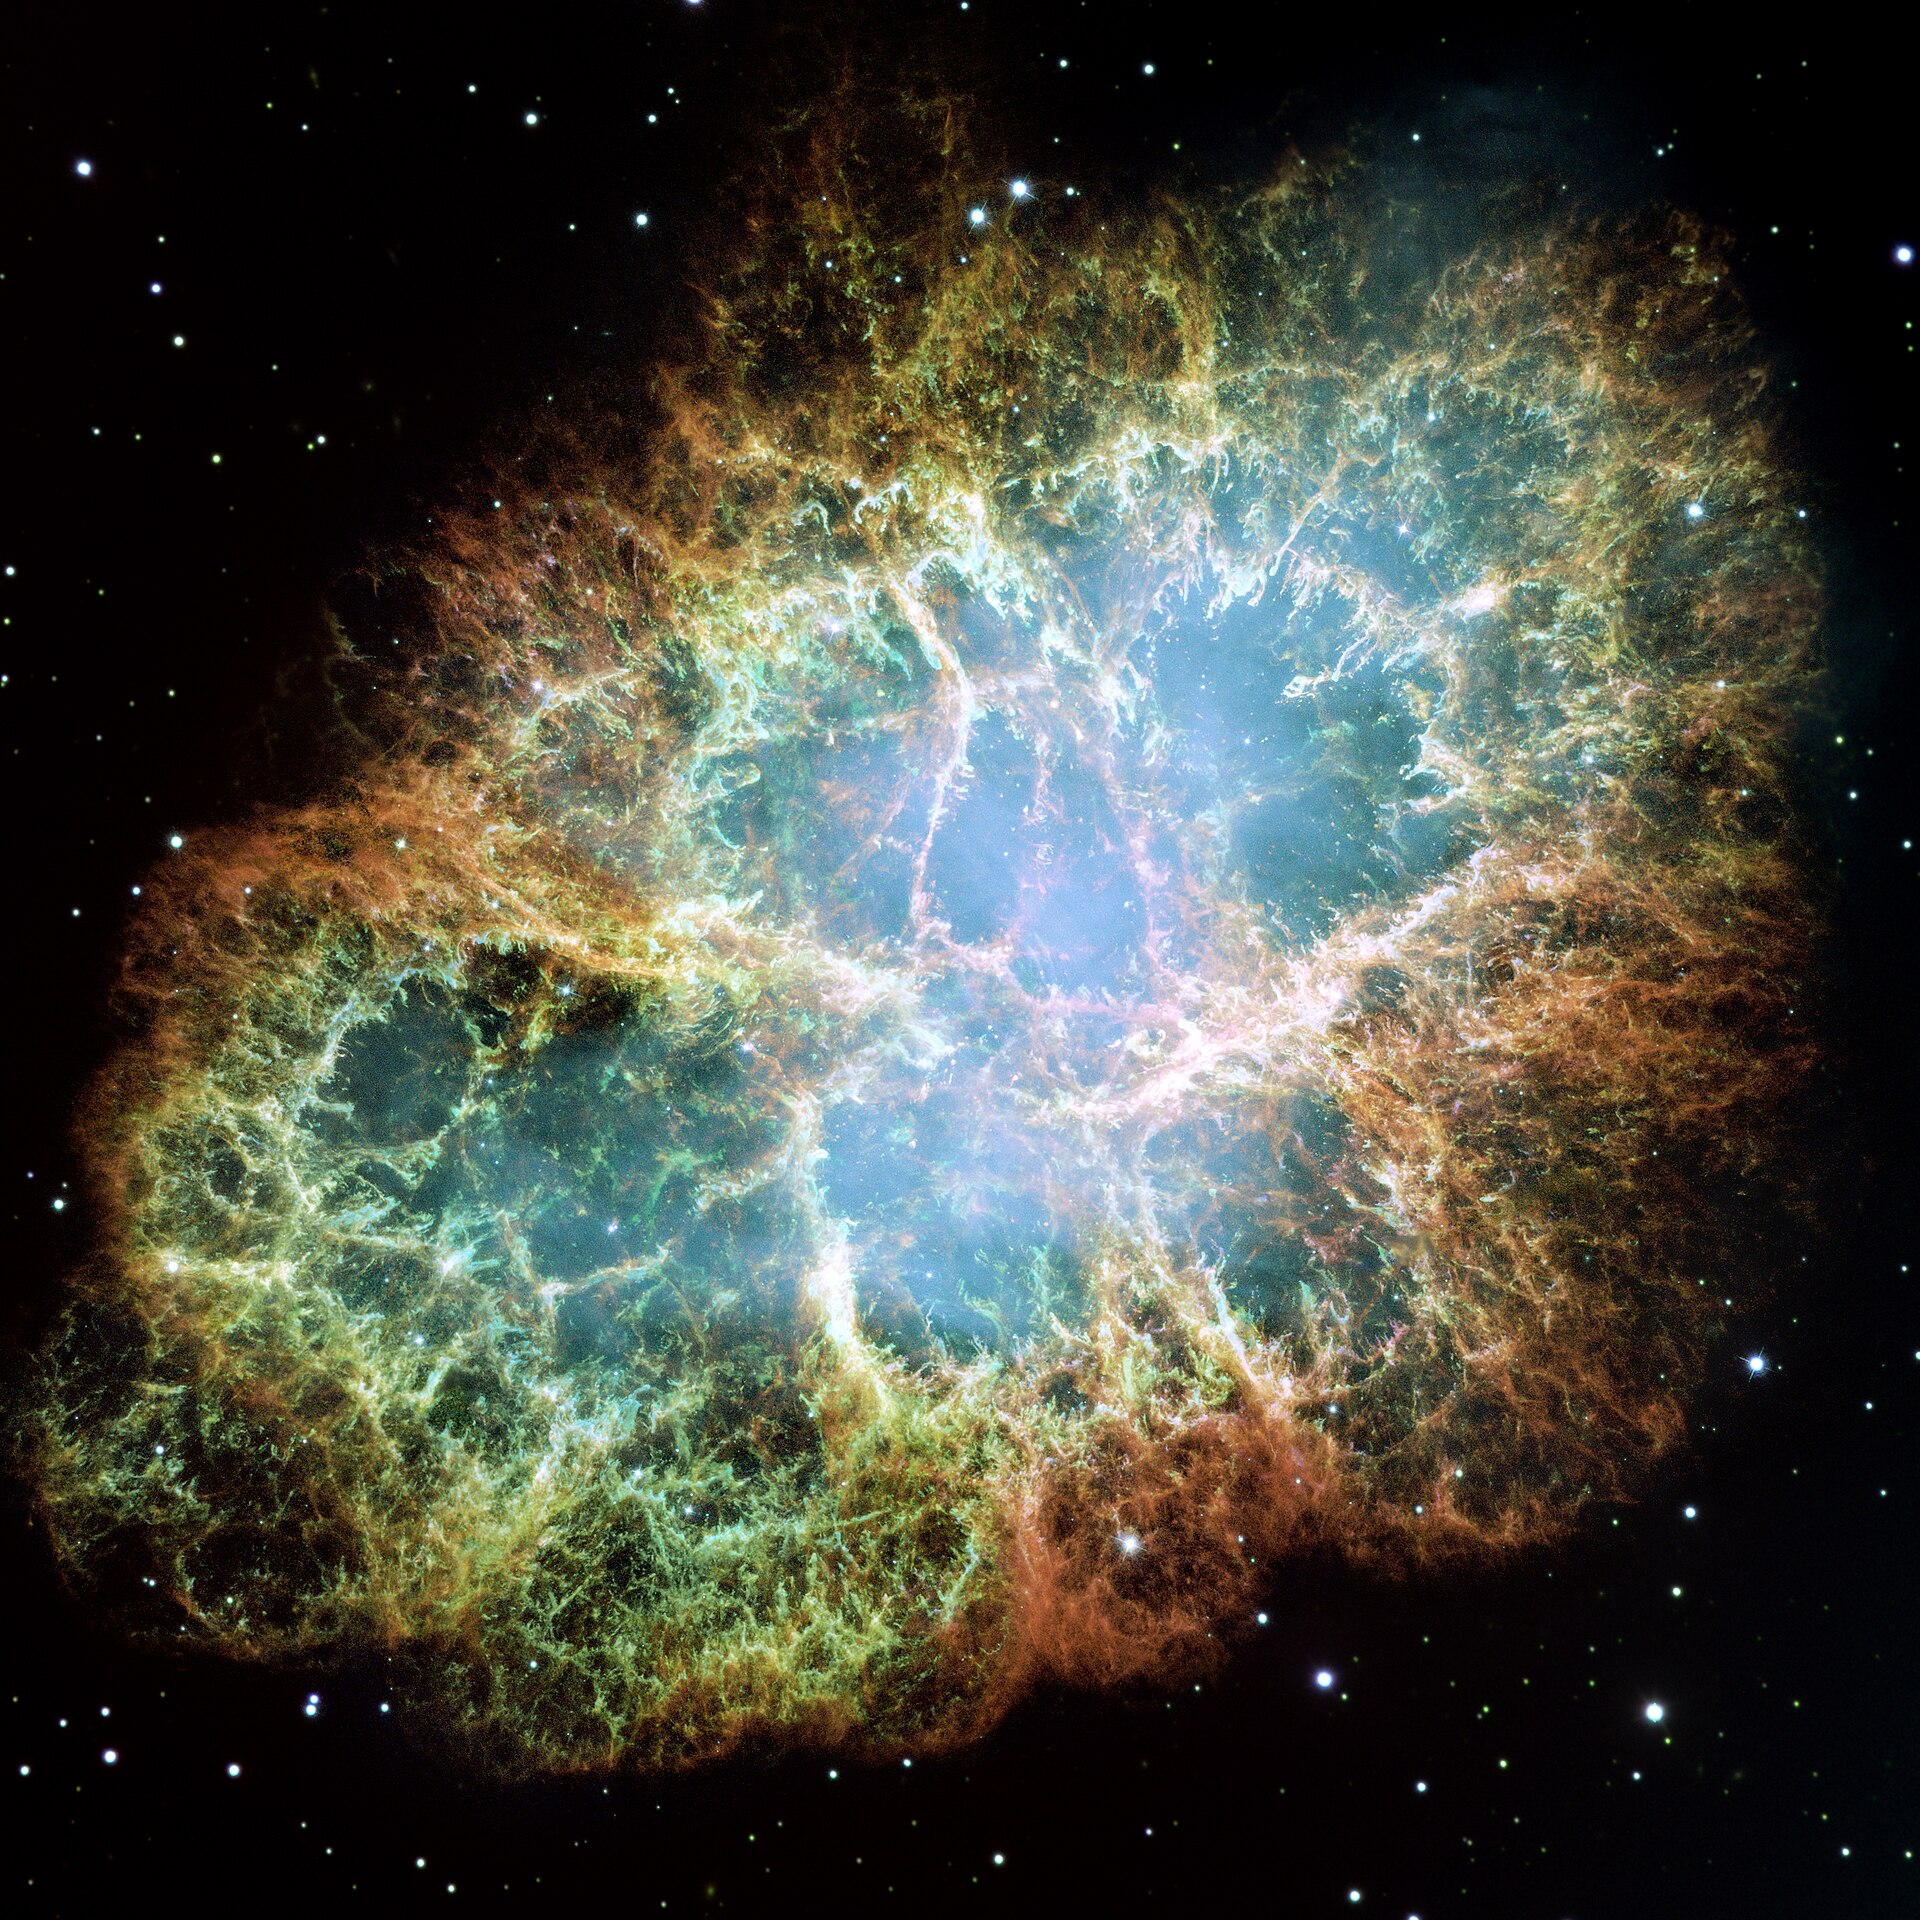
\includegraphics[width=0.6\linewidth]{images/book5/photo-crab-nebula.jpg}

{\small La nébuleuse du Crabe (NASA, ESA, J. Hester et A. Loll, domaine public)~: les débris de la supernova de 1054, toujours en expansion, avec le phare à la milliseconde d'une \omterm{prop:b3:astrophysics:compact}{étoile à neutrons} en son cœur --- le problème du week-end, photographié neuf siècles plus tard.}
\end{omfigure}

\section{Problème~: la nuit où l'étoile est morte}

\begin{problem}\label{pb:b3:astrophysics:1}
\emph{La nuit où l'étoile est morte.} Le 23 février 1987, une
supergéante bleue du Grand Nuage de Magellan --- $d \approx
\qty{50}{kpc} \approx \qty{1.5e21}{m}$ --- devint SN~1987A, la
supernova la plus proche en quatre siècles. Des heures \emph{avant}
qu'aucun télescope ne la voie s'aviver, trois détecteurs souterrains
ont compté deux douzaines de neutrinos. Vous reconstituez cette nuit
à partir des premiers principes.

\medskip\noindent\textbf{Partie I --- L'étoile qui fut.}

\begin{enumerate}
  \item Le progéniteur pesait ${\sim}20\,M_\odot$. À l'aide de la
        loi d'échelle de \cref{exo:b3:astrophysics:4}, estimer sa
        durée de vie et comparer à celle du Soleil.
  \item À son dernier jour, l'étoile était un oignon~: des couches
        de H, He, C, O, Si autour d'un cœur de fer. Pourquoi chaque
        combustible successif exige-t-il un cœur plus chaud~?
  \item Pourquoi la séquence s'arrête-t-elle définitivement au fer~?
        (\cref{prop:b3:nuclear-physics:binding}.)
  \item Le cœur de fer inerte croît vers $1.4\,M_\odot$. Qu'a de
        particulier ce nombre, et quelle pression y fait défaut~?
  \item La combustion du silicium soutient l'étoile pendant environ
        un \emph{jour}~: que dit cela de l'accélération de
        l'horloge d'une étoile vers la fin~?
  \item Une fois le soutien de pression perdu, combien de temps
        dure à peu près la chute libre, pour un cœur de masse
        volumique $\sim\qty{e12}{kg/m^3}$
        ($t \sim 1/\sqrt{G\rho}$)~?
\end{enumerate}

\medskip\noindent\textbf{Partie II --- L'éclair de neutrinos.}

\begin{enumerate}[resume]
  \item Le cœur ($M \approx 1.4\,M_\odot = \qty{2.8e30}{kg}$)
        s'effondre à $R \approx \qty{12}{km}$~: calculer l'énergie
        gravitationnelle libérée, $E \sim GM^2/R$.
  \item Comparer à la lumière d'un milliard de soleils brillant
        pendant un mois ($L \sim 10^{9}L_\odot$ durant
        $\qty{2.6e6}{s}$)~: montrer que les photons sont une erreur
        d'arrondi --- où passent les 99\,\%, et pourquoi seuls les
        neutrinos peuvent-ils quitter promptement un cœur en
        effondrement~?
  \item Répartir $E \approx \qty{3e46}{J}$ sur une sphère de
        rayon \qty{1.5e21}{m}~: calculer la fluence en énergie à la
        Terre.
  \item Avec $\sim\qty{15}{MeV}$ par neutrino, calculer la fluence
        en nombre (neutrinos par \unit{m^2}).
  \item Un détecteur contient \qty{2000}{t} d'eau~:
        ${\sim}1.5\times10^{32}$ protons libres. Avec une
        probabilité d'interaction par proton de
        $\sigma \approx \qty{1e-46}{m^2}$ par antineutrino
        (donnée), estimer le comptage attendu --- et comparer aux
        onze qu'un détecteur a enregistrés.
  \item Les neutrinos ont battu la lumière de plusieurs heures.
        Expliquer les deux horloges~: qu'est-ce qui retarde les
        photons (où naît réellement l'éclaircissement~?), et que dit
        la \omterm{def:b3:relativistic-kinematics:event}{quasi-simultanéité} sur la masse et la vitesse du
        neutrino~?
  \item Vingt-cinq neutrinos comptés~: dites, en une phrase
        chacune, deux choses qu'ils ont confirmées de la théorie des
        supernovae.
\end{enumerate}

\medskip\noindent\textbf{Partie III --- Ce qui reste.}

\begin{enumerate}[resume]
  \item Calculer la masse volumique moyenne du résidu de
        \qty{12}{km} et $1.4\,M_\odot$ et comparer à la densité
        nucléaire de
        \cref{def:b3:nuclear-physics:nuclide}.
  \item Le cœur du progéniteur tournait une fois par 30 jours à
        $R \sim \qty{e5}{km}$~: estimer la période du résidu.
  \item Son champ magnétique, gelé dans le flux, est amplifié par
        $(R_0/R)^2$~: à partir de \qty{e-2}{T}, calculer le champ de
        surface.
  \item Expliquer le phare~: qu'est-ce qui balaie, qu'est-ce qui
        rayonne en faisceau, et pourquoi le pulsar du Crabe (né en
        1054, chroniqué comme une «~étoile invitée~» visible de
        jour) clignote-t-il encore trente fois par seconde~?
  \item Si le résidu avait dépassé ${\sim}3\,M_\odot$~: calculer
        $R_{\text{s}}$ pour $3\,M_\odot$ et dites son destin.
  \item La chronométrie des pulsars est stable à $10^{-15}$~:
        nommer un usage physique d'une horloge aussi bonne, tournant
        dans le ciel.
\end{enumerate}

\medskip\noindent\textbf{Partie IV --- Ce que cela signifie.}

\begin{enumerate}[resume]
  \item L'oxygène que vous respirez et le fer de votre sang~:
        retracer la biographie de chaque atome en deux phrases, de
        l'hydrogène du Big Bang à votre circulation sanguine.
  \item Les supernovae de type Ia (des \omterm{ex:b3:quantum-statistics:dwarf}{naines blanches} poussées
        au-delà de $M_{\text{Ch}}$) détonent toutes à la même masse,
        donc à un éclat presque identique. Expliquer pourquoi cela
        en fait des \emph{chandelles standard}, et comment le
        diagramme de \cref{def:b3:astrophysics:hubble} se construit
        à partir d'elles.
  \item En 1998, des supernovae Ia lointaines se sont révélées
        \emph{plus faibles} que ne le prédit la droite de Hubble~:
        énoncer la conclusion qui a valu le prix Nobel 2011.
  \item Estimer en années la distance parcourue par la lumière de
        SN~1987A à son arrivée --- et noter ce qui se passait sur
        Terre quand elle est partie.
  \item Les neutrinos du Grand Nuage vous ont traversé aussi (comme
        tous les vivants de ce jour-là). Combien environ ont
        traversé chaque être humain (${\sim}\qty{0.03}{m^2}$)~?
        Quelqu'un l'a-t-il senti
        (\cref{exo:b3:particle-physics:10})~?
  \item Refermer le grand livre en quatre lignes~: une étoile tenue
        en équilibre pendant dix millions d'années par l'effet
        tunnel~; un effondrement payé en neutrinos~; un cadavre
        soutenu par Pauli~; et les débris --- le lecteur compris ---
        toujours emportés par l'expansion de Hubble.
\end{enumerate}
\end{problem}
